\documentclass{article}

\usepackage{ross}
\newcommand{\labelthis}[1]{\addtocounter{equation}{1}\tag{\theequation}\label{#1}}
\usepackage{pgfplots}
\fancyhdr

\begin{document}
\makeheading{Energy in the genus zero case}
Hitchin has a formula for the energy, given in Theorem 13.17. In the nonconformal case if the differentials are expanded as
\[
\Theta = \frac{d\zeta}{\zeta^2}(\theta_{-2} + \theta_0\zeta^2 + \dots)
\]
and similiarly for $\tilde \Theta$ then the energy is given as $E = 4i(\theta_0 \tilde \theta_{-2} - \tilde \theta_0 \theta_{-2})$. Our preferred form for the differentials is
\[
  \Theta = \frac{d\zeta}{\zeta^2\eta}b(\zeta)
\]
for a polynomial $b$ of degree $g+3$, where $g$ is the genus of the spectral curve $\eta^2 = P(\zeta)$. About $\zeta=0$, there is a series expansion for $\eta$ (subscripts denoting coefficients of a series or polynomial)
\[
  1/\eta \sim \frac{1}{\sqrt{P_0}}\left(1 - \frac{1}{2}\frac{P_1}{P_0}\zeta + \frac{3P_1^2 - 4P_0P_2}{8P_0^2}\zeta^2\dots\right)
\]
and so we have
\[
  \Theta \sim \frac{d\zeta}{\zeta^2}\frac{1}{\sqrt{P_0}}\left[ b_0 + \zeta\left( b_1 - \frac{1}{2}\frac{P_1}{P_0}b_0 \right) + \zeta^2\left( b_2 - \frac{1}{2}\frac{P_1}{P_0}b_1 + \frac{3P_1^2 - 4P_0P_2}{8P_0^2}b_0 \right) + \dots\right]
\]
from which we see that $\theta_{-2} = b_0 / \sqrt P_0$ and that
\[
  \theta_0 = \frac{1}{\sqrt{P_0}}\left[b_2 - \frac{1}{2}\frac{P_1}{P_0}b_1 + \frac{3P_1^2 - 4P_0P_2}{8P_0^2}b_0\right] = \frac{1}{\sqrt{P_0}}\left[b_2 - A b_0\right]
\]
for some constant $A$, using the fact that $\Theta$ has no residues to eliminate $b_1$. Putting this into the energy formula, we arrive at the following version
\[
  E = \frac{4i}{P_0} (b_2 \tilde b_0 - \tilde b_2 b_0)
\]
Now we specialise to the genus zero case. Here, the $b$ polynomial is only degree $3$ and so the reality condition forces $b_2 = \bar b_1$, which is itself a multiple of $\bar b_0$. But we can be even more explict that this. If we choose integers $n,m,\tilde n, \tilde m$ and a root $\alpha$ in the unit disc, then we write
\begin{align*}
r &= \sqrt{ 1 + \alpha\bar \alpha + \alpha + \bar \alpha} \\
s &= \sqrt{ 1 + \alpha\bar \alpha - \alpha - \bar \alpha} \\
a &= \frac{\pi}{2}\left( \frac{n}{r} + i\frac{m}{s} \right) \\
\tilde a &= \frac{\pi}{2}\left( \frac{\tilde n}{r} + i\frac{\tilde m}{s} \right)\\
b_0 &= - \alpha \bar a \\
\tilde b_0 &= - \alpha \bar{\tilde a} \\
P(\zeta) &= -\alpha + (1+\alpha\bar \alpha)\zeta - \bar \alpha\zeta^2 \\
& \\
E &= 4i \frac{1}{P_0}\frac{1}{2}\frac{P_1}{\overline P_0}\frac{\pi^2}{4}\frac{-2i}{rs}(m\tilde n - n\tilde m) \\
&= \pi^2\frac{P_1}{rs}(m\tilde n - n\tilde m)
\end{align*}
A reasonable question to ask is, if one has a path of spectral data (in this case a choice of four integers and a path $\alpha(t)$), when does this path preserve the energy of the corresponding harmonic maps?
\[
\dot E = 0 \Rightarrow \left(\Real\alpha\right)\left( \Real\frac{\dot \alpha}{1-\alpha^2} \right) = 0
\]
The left factor corresponds to the imaginary axis. The second factor corresponds to a circle centered on the real axis that cuts the unit circle perpedicularly. In other words, $\dot E$ is zero precisely when $\alpha$ moves on an arc that preserves $\tau$; such arcs form a family of hyperbolic geodesics that foliate the unit disc.

\section*{Discussion}
Why $E$ and $\tau$ are linked like this must be related to the fact that $\tilde b_0 = \tau b_0$, but I haven't managed to derive a neat relation.

Below is a plot of the energy as a function over $\alpha = x + i y$. There are obvious singularities at $\alpha=1,-1$, which is the limit as the torus we are mapping from becomes infinitely stretched. The arcs mentioned above are level curves for this graph. What is curious though is that these do not appear to be critical points of the energy function. My only guess as to what is happening, is that they are critical points when considered in the infinite dimensional space of functions, but not in this finite subspace of spectral genus zero harmonic maps (not sure exactly how that would work).

\begin{center}
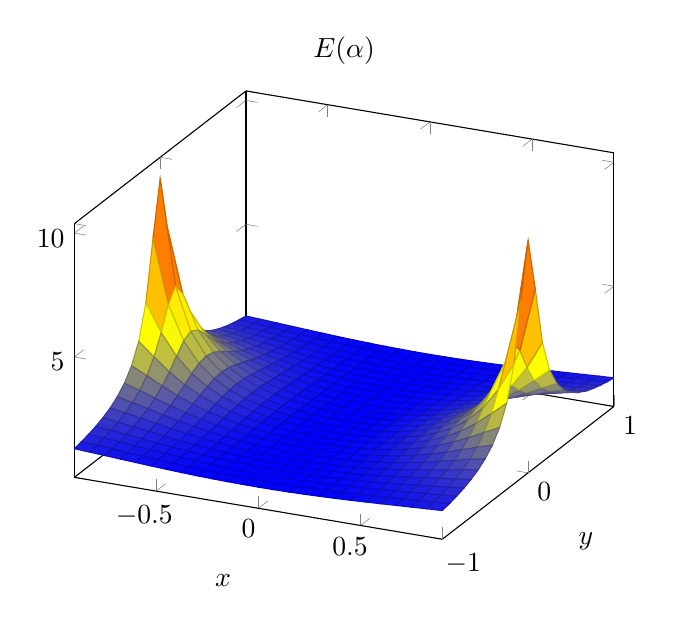
\begin{tikzpicture}
\begin{axis}[
    title={$E(\alpha)$},
    xlabel=$x$, ylabel=$y$,
]
\addplot3[
	surf,
	domain=-0.9:0.9,
	domain y=-1:1,
]
	{(1+x^2 + y^2)/(sqrt((1-x^2+y^2)^2 + 4*x^2 *y^2))};
\end{axis}
\end{tikzpicture}
\end{center}

\end{document}
